%%%%%%%%%%%%%%%%%%%%%%%%%%%%%%%%%%%%%%
% Numerical Linear Algebra class 2022 
% Solutions to Sheet 8
%%%%%%%%%%%%%%%%%%%%%%%%%%%%%%%%%%%%%%

\begin{SolutionSheet}[\ref{sheet8}]

  \begin{Solution}
    \begin{enumerate}[(a)]
    \item Sample calculation of LU factorization in
      \lstinline{./programs/lu.py}. Sparsity patterns in figure below.

      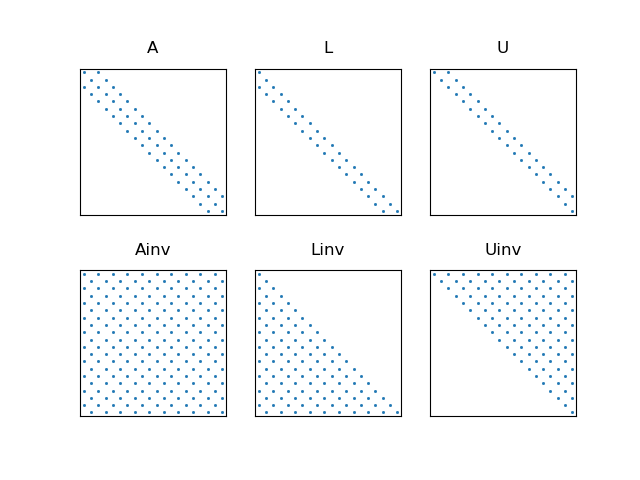
\includegraphics[width=0.8\textwidth]{figures/lu-decomposition-of-sparse-matrix}
    \item The width of the zero diagonals gets transported to the
       matrices of the LU factorization

      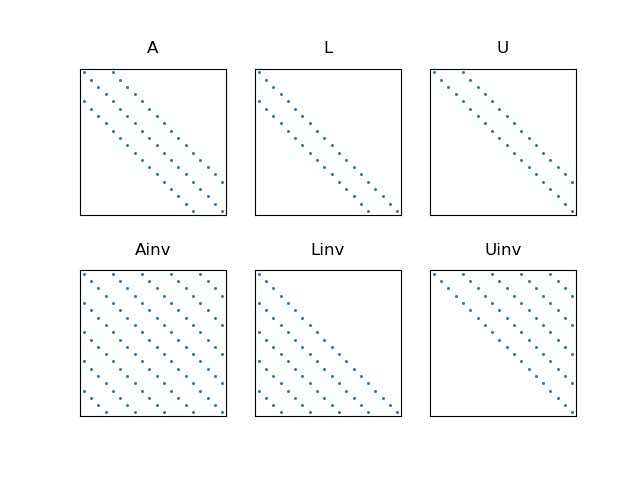
\includegraphics[width=0.8\textwidth]{figures/lu-decomposition-of-sparse-matrix-off4}
    \item The inverse is dense up to the zero diagonals that get
      scattered over the whole inverse
    \end{enumerate}

    
  \end{Solution}

  \begin{Solution}[{\cite[P-5.1 b]{Saad00}}]
    \hfill\\
    Hint 1:
    \begin{gather*}
      \scal(\mata\vd^{(k+1)},\vd^{(k+1)})
      =\scal(\mata\vd^{(k)},\vd^{(k)})
      -\frac{\scal(\vr^{(k)},\ve_i)^2}{a_{ii}}
    \end{gather*}

    Hint 2:
    \begin{gather*}
      \abs{\ve_i^T \vr^{(k)}} \geq n^{-\nfrac12}\norm{\vr^{(k)}}_2
    \end{gather*}

    With the help of hint 1 and 2 we get
    \begin{align*}
      \norm{\vd^{(k+1)}}_{\mata}^2
      = \scal(\mata\vd^{(k+1)},\vd^{(k+1)})
      &\stackrel{\text{Hint 1}}{=}
        \scal(\mata\vd^{(k)},\vd^{(k)})
        - \frac{\scal(\vr^{(k)},\ve_i)^2}{a_{ii}}
      \\
      &=
        \left( 1 - \frac{\scal(\vr^{(k)},\ve_i)^2}{a_{ii}}
              \frac1{\scal(\mata\vd^{(k)},\vd^{(k)})} \right)
        \norm{\vd^{(k)}}_{\mata}^2
      \\
      &\stackrel{\text{Hint 2}}{\leq}
        \left( 1 - \frac{1}{n a_{ii}}
              \frac{\norm{\vr^{(k)}}_2^2}{\scal(\mata\vd^{(k)},\vd^{(k)})} \right)
        \norm{\vd^{(k)}}_{\mata}^2
    \end{align*}
    The result follows by the following two estimates of Rayleigh quotients:
    \begin{gather*}
      a_{ii} = \scal(\mata\ve_i,\ve_i) = \frac{\scal(\mata\ve_i,\ve_i)}{\scal(\ve_i,\ve_i)}
      \le \lambda_{\max},
    \end{gather*}
    and
    \begin{gather*}
      \frac{\scal(\mata\vd^{(k)},\vd^{(k)})}{\norm{\vr^{(k)}}^2}
      = \frac{\scal(\vr^{(k)},\mata^{-1}\vr^{(k)})}{\norm{\vr^{(k)}}^2}
      \le \lambda_{\max}(\mata^{-1})
      = \frac1{\lambda_{\min}}.
    \end{gather*}

    Final remarks:\\
    1. Since $\ve_i\in K=L$, it holds the Galerkin-orthogonality
    \begin{align*}
      \scal(\vr^{(k)}-\alpha\mata \ve_i,\ve_i) = 0,
    \end{align*}
    where according to Example 2.3.10
    \begin{gather*}
      \alpha = \frac{\scal(\vr^{(k)},\ve_i)}{\scal(\mata\ve_i,\ve_i)}
      = \frac{\scal(\vr^{(k)},\ve_i)}{a_{ii}}
      .
    \end{gather*}
    This would have been used to show hint 1.

    2. To show hint 2, notice that by the choice of $i$ as maximal
    value of the residual vector
    \begin{align*}
      \norm{\vr^{(k)}}_2
      \leq \sqrt{n} \norm{\vr^{(k)}}_{\infty}
      = \sqrt{n} \abs{\ve_i^T\vr^{(k)}}
    \end{align*}

  \end{Solution}

  \begin{Solution}
  \end{Solution}

  \begin{Solution}[Programming]
    C++ sample code \lstinline{./programs/steepest-decent.cc} without
    assembling the system matrix.

    Convergence rate (Definition 2.2.18 in lecture notes).  As can be
    seen in the plot, the convergence of the steepest decent method is
    sublinear.

    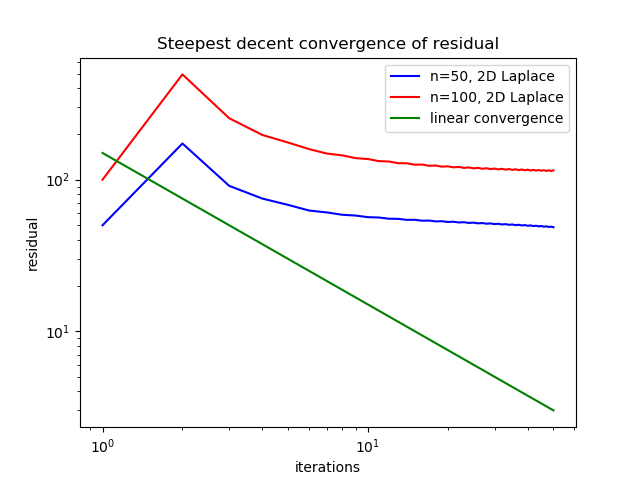
\includegraphics[width=\textwidth]{figures/laplace-steepest-decent}
  \end{Solution}

\end{SolutionSheet}


%%% Local Variables: 
%%% mode: latex
%%% TeX-master: "main"
%%% End: 
